%%%%%%%%%%%%%%%%%%%%%%%%%%%%%%%%%%%%%%%%%%%%%%%%%%%%%%%%%
\section{2D Unsteady Uniform Property: Convecting Decaying Taylor Vortex}
%%%%%%%%%%%%%%%%%%%%%%%%%%%%%%%%%%%%%%%%%%%%%%%%%%%%%%%%%

Verification of first-order and second-order temporal accuracy for the
CVFEM and EBVC formulation in Nalu is performed using the method of manufactured 
solution (MMS) technique. For the unsteady isothermal, uniform laminar physics set,
the exact solution of the convecting, decaying Taylor vortex is used.

\begin{equation}
  u = u_o - cos(\pi(x-u_ot)) sin(\pi(y-v_ot))e^{-2.0\omega t}
\label{advConvTV_u}
\end{equation}

\begin{equation}
  v = v_o + sin(\pi(x-u_ot)) cos(\pi(y-v_ot))e^{-2.0\omega t} 
\label{advConvTV_v}
\end{equation}

\begin{equation}
  p = -\frac{p_o}{4}(cos(2\pi(x-u_ot)) + cos(2\pi(y-v_ot)))e^{-4\omega t}
\label{advConvTV_p}
\end{equation}

In this study, the constants $u_o$, $v_o$, and $p_o$ are all assigned values of $1.0$,
and the viscosity $\mu$ is set to a
constant value of $0.001$. The value of $\omega$ is $\pi^2\mu$. This particular viscosity value 
results in a maximum cell reynolds number of twenty.  

\subsection{Temporal Order Of Accuracy Results}
The temporal order of accuracy for the first order backward Euler and second order BDF2
are outlined in Figure~\ref{fig:fo4thTstep} and Figure~\ref{fig:so4thTstep}. Each of these
simulations used a hybrid factor of zero to ensure pure second order central usage. A
fixed Courant number of two was used for each of the three meshes (100x100, 200x200 and 400x400).
The simulation was run out to 0.2 seconds and $L_2$ error norms were computed. The standard
fourth order pressure stabilization scheme with time step scaling is used. This scheme is also
known as the standard incremental pressure, approximate pressure projection scheme.

Two other pressure projection schemes have been evaluated in this study. Each represent a 
simplification of the standard pressure projection scheme. Figure~\ref{fig:hybridTstep} outlines
three projection schemes: the first is when the projected nodal gradient appearing in the fourth-order 
pressure stabilization is lagged while the second is the classic pressure-free pressure approximate projection 
scheme with second order pressure stabilization. The third is the baseline fourth-order incremental pressure projection 
scheme. The error plots demonstrate that lagging the projected nodal 
gradient for pressure retains second order accuracy. However, as expected the pressure
free pressure projection scheme is confirmed to be first order accurate given the first order splitting error noted in this fully implicit momentum solve.

The Steady Taylor Vortex will be used to verify the spatial accuracy for the full set of advection
operators supported in Nalu.
 
\begin{figure}
\centerline{\includegraphics[width=0.8\textwidth]{figures/convTaylorVortexFO.pdf}}
\caption{Error norms as a function of timestep size for the $u$ and $v$
component of velocity using fourth order pressure stabilization with timestep scaling, backward Euler}
\label{fig:fo4thTstep}
\end{figure}

\begin{figure}
\centerline{\includegraphics[width=0.8\textwidth]{figures/convTaylorVortexSO.pdf}}
\caption{Error norms as a function of timestep size for the $u$ and $v$
component of velocity using fourth order pressure stabilization with timestep scaling, BDF2}
\label{fig:so4thTstep}
\end{figure}

\begin{figure}
\centerline{\includegraphics[width=0.8\textwidth]{figures/convTaylorVortexSO_ElemLagElemPf.pdf}}
\caption{Error norms as a function of timestep size for the $u$ and $v$
component of velocity using the lagged projected nodal pressure gradient and pressure-free pressure projection scheme; all with with timestep scaling, BDF2}
\label{fig:hybridTstep}
\end{figure}

\section{Higher Order 2D Steady Uniform Property: Taylor Vortex}

A higher order unstructured CVFEM method has been developed by Domino~\cite{Domino:2014}. 
A 2D structured mesh study demonstrating second order time and third order in space scheme 
has been demonstrated. The below work has emphasis on unstructured meshes.

\subsection{Source Term Quadrature}
Higher order accuracy is only demonstrated on solutions with source terms when a fully integrated
approach is used. Lumping the source term evaluation is a second order error and is fully noted in
the MMS study (not shown).

\subsection{Projected nodal gradients}
Results show that one must use design order projected nodal gradients. Figure~\ref{fig:pngTempMMS} demonstrates 
a code verification result for a steady thermal manufactured solution comparing lumped and consistent mass matrix approaches for the projected nodal gradient on a quadratic tquad mesh. In the lumped approach, a simple explicit algorithm is processed while for the consistent approach, a simple mass matrix inversion equation must be solved. The lumped approach is first order while the consistent approach retains the expected second order as the projected nodal gradient is expected to be order $P$. Both Dirichlet and periodic domains display the same order of convergence.

\begin{figure}
\centerline{\includegraphics[width=0.8\textwidth]{figures/ho_heatCondMMM_dtdx.pdf}}
\caption{Error norms as a function of mesh size for a CMM and LMM projected 
nodal gradient on a quadratic tquad mesh.}
\label{fig:pngTempMMS}
\end{figure}

\subsection{Momentum and Pressure}
The steady taylor vortex exact solution was run on a quadratic tquad mesh. Figure~\ref{fig:hoSTVMMS} demonstrates the order of accuracy for projected nodal gradients (pressure) and the velocity field (x-component). Second order accuracy for the projected nodal gradient (pressure) and third order for the velocity field is realized when the consistent mass matrix approach is used for the projected nodal pressure gradient. Note that this term is used in the pressure stabilization approach. However, order of convergence for the projected nodal pressure gradient and velocity field is compromised when the lumped mass matrix approach is used for the pressure stabilization term. Note that both approaches use the fully integrated pressure gradient term in the momentum equation (i.e., $\int p n_i dS$). Therefore, the reduced order of integration for the projected nodal pressure gradient has consequence on the velocity field order of convergence.
 
Again, dirichlet (inflow) and periodic domains display the same order of convergence.

\begin{figure}
\centerline{\includegraphics[width=0.8\textwidth]{figures/ho_stvUandDpDx.pdf}}
\caption{Error norms as a function of mesh size for the Steady Taylor Vortex 
momentum and pressure gradient field.}
\label{fig:hoSTVMMS}
\end{figure}

%%%%%%%%%%%%%%%%%%%%%%%%%%%%%%%%%%%%%%%%%%%%%%%%%%%%%%%%%
\section{3D Steady Non-isothermal with Buoyancy}
%%%%%%%%%%%%%%%%%%%%%%%%%%%%%%%%%%%%%%%%%%%%%%%%%%%%%%%%%

Building from the basic functional form of the Taylor Vortex,
a non-isothermal solution (momentum, pressure and static enthalpy)
is manufactured as follows:

\begin{eqnarray}
  u &=& -u_o cos(a \pi x) sin(a \pi y ) sin(a \pi z) \nonumber \\
  v &=& +v_o sin(a \pi x) cos(a \pi y ) sin(a \pi z) \nonumber \\
  w &=& -w_o sin(a \pi x) sin(a \pi y ) cos(a \pi z) \nonumber \\
  p &=& -\frac{p_o}{4}( cos(2 a \pi x) + cos(2 a \pi y ) + cos(2 a \pi z) )  \nonumber \\
  h &=& +h_o cos(a_h \pi x) cos(a_h \pi y ) cos(a_h \pi z)  \nonumber \\
\label{3dNonIso}
\end{eqnarray}
%
The equation of state is simply the ideal gas law, 
\begin{equation}
  \rho = \frac{P^{ref} M}{R T}
\label{idealGasEOS}
\end{equation}

The simulation is run on a three-dimensional domain ranging from -0.05:+0.05 with
constants $a, a_h, M, R, C_p, P^{ref}, T_{ref}, Pr, \mu$ equal to 
(20, 10, 30, 10, 0.01, 100, 300, 0.8, 0.00125), respectively.

At reference conditions, the density is unity. The effects of buoyancy are also provided 
by an arbitrary gravity vector of magnitude of approximately ten, $g_i = (-5, 6, 7)^T$. On this domain, 
the enthalpy ranges from zero to unity. Given the reference values, the temperature 
field ranges from 300K to 400K which is designed to mimic a current LES non-isothermal 
validation suite.

Edge- and element-based discretization (P=1) demonstrate second order convergence
in the $L_2$ norm for u, v, w and temperature. This test is captured within the 
variableDensityMMS regression test suite.

%%%%%%%%%%%%%%%%%%%%%%%%%%%%%%%%%%%%%%%%%%%%%%%%%%%%%%%%%
\section{3D Steady Non-uniform with Buoyancy}
%%%%%%%%%%%%%%%%%%%%%%%%%%%%%%%%%%%%%%%%%%%%%%%%%%%%%%%%%

Building from the basic functional form of the Taylor Vortex,
a non-uniform solution (momentum, pressure and mixture fraction)
is manufactured as follows:

\begin{eqnarray}
  u &=& -u_o cos(a \pi x) sin(a \pi y ) sin(a \pi z) \nonumber \\
  v &=& +v_o sin(a \pi x) cos(a \pi y ) sin(a \pi z) \nonumber \\
  w &=& -w_o sin(a \pi x) sin(a \pi y ) cos(a \pi z) \nonumber \\
  p &=& -\frac{p_o}{4}( cos(2 a \pi x) + cos(2 a \pi y ) + cos(2 a \pi z) )  \nonumber \\
  z &=& +z_o cos(a_z \pi x) cos(a_z \pi y ) cos(a_z \pi z)  \nonumber \\
\label{3dNonIso}
\end{eqnarray}
%
The equation of state is simply the standard inverse mixture fraction 
property expression for density, 
\begin{equation}
  \rho = \frac{1} {\frac{z}{rho^P} + \frac{1-z}{rho^S} }
\label{idealGasEOS}
\end{equation}

The simulation is run on a three-dimensional domain ranging from -0.05:+0.05 with
constants $a, a_z, \rho^p, \rho^s, Sc, \mu$ equal to (20, 10, 0.1, 1.0, 0.8, 0.001),
respectively.

At reference conditions, the density is that of the primary condition (0.1). 
The effects of buoyancy are also provided by an arbitrary gravity vector 
of magnitude of approximately ten, $g_i = (-5, 6, 7)^T$. On this domain, the mixture 
fraction ranges from zero to unity. This test case is designed to support 
the helium plume DNS study with primary and secondary density values of helium
and air, respectively.

Edge- and element-based discretization (P=1) demonstrate second order convergence
in the $L_2$ norm for u, v, w and mixture fraction. This test is captured within the 
variableDensityMMS regression test suite.

%%%%%%%%%%%%%%%%%%%%%%%%%%%%%%%%%%%%%%%%%%%%%%%%%%%%%%%%%
\section{2D Steady Laplace Operator}
%%%%%%%%%%%%%%%%%%%%%%%%%%%%%%%%%%%%%%%%%%%%%%%%%%%%%%%%%
The evaluation of the low-Mach Laplace (or diffusion operator) is of great interest to the core supported application
space. Although the application space for Nalu is characterized by a highly turbulent flow, the usage of an approximate 
pressure projection scheme always makes the chosen Laplace form important. Although the element-based scheme is expected 
to be accurate, it can be problematic on high aspect ratio meshes as element-based schemes are not gauranteed to be monotonic 
for aspect ratios as low as $sqrt(2)$ for FEM-based schemes and $sqrt(3)$ for CVEM-based approaches (both when using standard 
Gauss point locations). Conversely, while the edge-based operator is accurate on high aspect ratio meshes, it suffers on skewed 
meshes due to both quadrature error and the inclusion of a non orthogonal correction (NOC). 

In order to assess the accuracy of the Laplace operator, a the two-dimensional MMS temperature solution 
is used. The functional temperature field takes on the following form:

\begin{equation}
  T = \frac{\lambda}{4} (cos(2 a \pi x) + cos(2 a \pi y)).
\label{advConvTV_u}
\end{equation}

The above manufactured solution is run on three meshes of domain size of 1x1. The domain was first meshed as a triangular mesh and
then converted to a tquad4 mesh. Therefore, non orthogonal correction (NOC) effects are expected for the edge-based scheme. 
In this study, both $\lambda$ and $a$ are unity. Either periodic or Dirichlet conditions are used for boundary conditions. 


A brief overview of the diffusion operator tested is now provided. For more details, consult the theory manual. The general 
diffusion kernel is as follows:

\begin{equation}
 -\int \Gamma \frac{\partial \phi}{\partial x_j} A_j.
\label{diffOp}
\end{equation}

The choice of the gradient operator at the integration point is a functin of the underlying method. For CVFEM,
the gradient operator is provided by the standard shape function derivatives,
\begin{equation}
 \frac{\partial \phi_{ip}}{\partial x_j} = \sum \frac{\partial N^{ip}_{j,k}} {\partial x_j} \phi_k.
\label{cvfemDerivative}
\end{equation}
For the edge-based scheme, a blending of an orthogonal gradient along the edge and a NOC is employed,
\begin{equation}
  \frac{\partial \phi_{ip}}{\partial x_j} = \bar{G_j\phi} + \left[ \left(\phi_R - \phi_L \right) 
- \bar{G_l\phi}dx_l \right] \frac{A_j}{A_k dx_k}.
\end{equation}
\label{generalGrad}
In the above equation, $G_j\phi$ is a projected nodal gradient. The general equation for this quantity is 
\begin{equation}
\int w_I G_j \phi {dV} = \int w_i \frac{\partial \phi}{\partial x_j}{dV}.
\label{PNG}
\end{equation}

Possible forms of this include either lumped or consistent mass (the later requires a global equation solve) with
either the full CVFEM stencil or the edge-based (reduced) stencil. The above equation can even be applied within 
the element itself for a simple, local integration step that provides a piecewise constant gradient over the element.

The simulation study is run with the following diffusion operators: 1) the standard CVFEM operator, 2) the edge-based
operator with CVFEM projected nodal gradients (NOC), 3) the edge-based operator with edge-based projected nodal gradients (NOC),
4) the edge-based operator without NOC correction, 5) the CVFEM operator with shifted integration points to the edge, and, lastly, 
6) a mixed edge/element scheme in which the orthogonal diffuion operator is edge-based while the NOC terms are based on the elemental 
CVFEM gradient (either evaluated at the given integration point or integrated over the element for a piecewise constant form).

The last operator is interesting in that it represents a candidate operator for the CVFEM pressure Poisson system when high aspect ratio 
meshes are used. Figure~\ref{fig:laplaceTquad} (a) outlines the convergence of the five above operators; shown are all of the standard 
norms (infinity, 1 and 2) for the R0, R1 and R2 mesh refinements. The results in the left side of the figure indicate that the edge-based 
scheme with NOC retains second-order convergence for all norms when the more accurate CVFEM projected nodal gradient is used (lumped only tested 
given its good results). Convergence is degraded with the edge-based scheme when NOC terms are either neglected or use the reduced edge-based 
projected nodal gradient. The CVFEM-based methods are second order accurate in the $L_1$ and $L_2$ norms, however, questionable 
results are noted in the $L_{oo}$ norm for all methods that include any shape function derivative for local or elemental piecwise constant 
gradient operators. Shifting the Gauss points from the standard subcontrol surface to the edges of the element (while still using shape function derivatives) 
is only problematic in the $L_{oo}$ norm (just as the standard CVFEM approach). The use of the mixed-approach with a piecewise constant gradient over the 
element demonstrates the same behavior as when using the integration point CVFEM gradient operator. Figure~\ref{fig:laplaceTquad} (b) outlines two more refinement meshes 
for the CVFEM operator (R3 and R4). Results indicate that the $L_{oo}$ norm is approaching second order accuracy.

\begin{figure}
  \centering
  \subfigure[R0, R1, and R2 refinement.]
  {
    \centerline{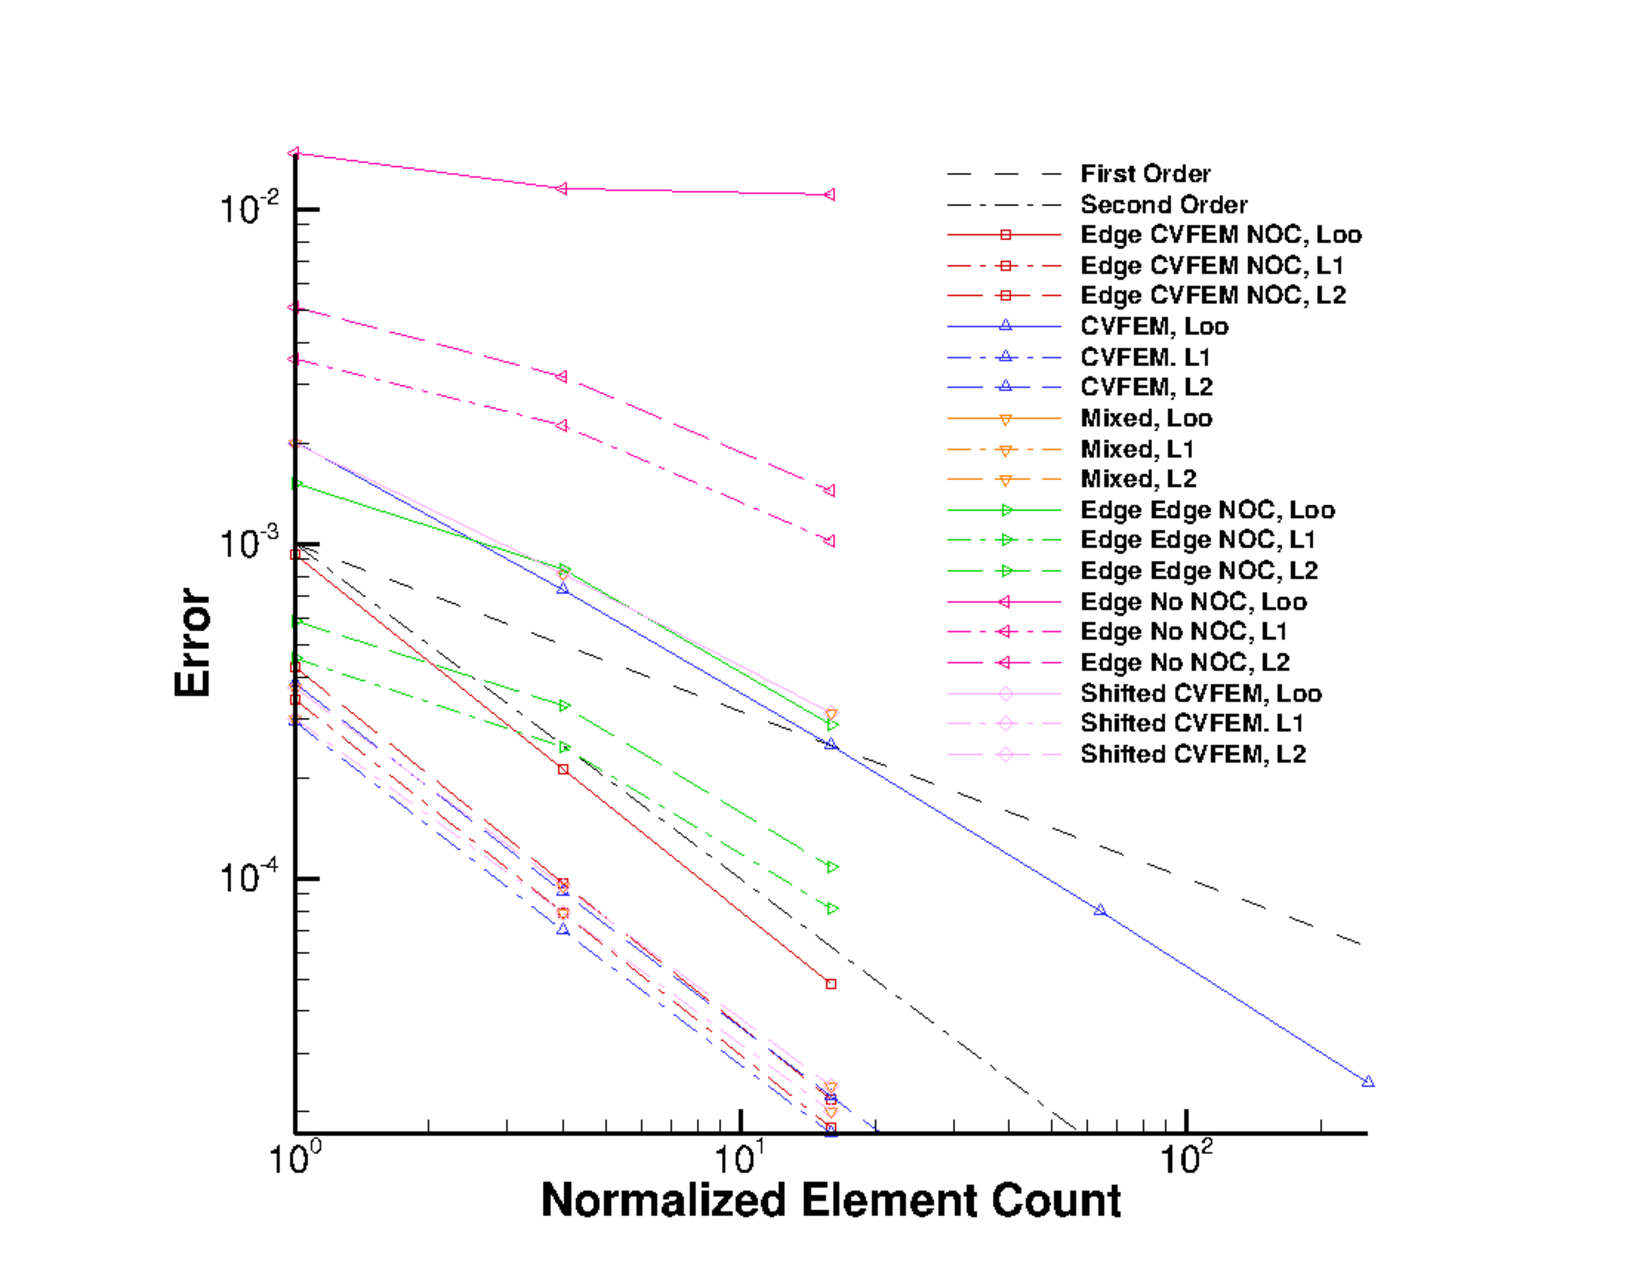
\includegraphics[width=0.8\textwidth]{figures/tquadLaplaceMMS.pdf}}
  }
  \subfigure [R0, R1, R2, R3, R4, and R4 refinementError for CVFEM.]
  {
    \centerline{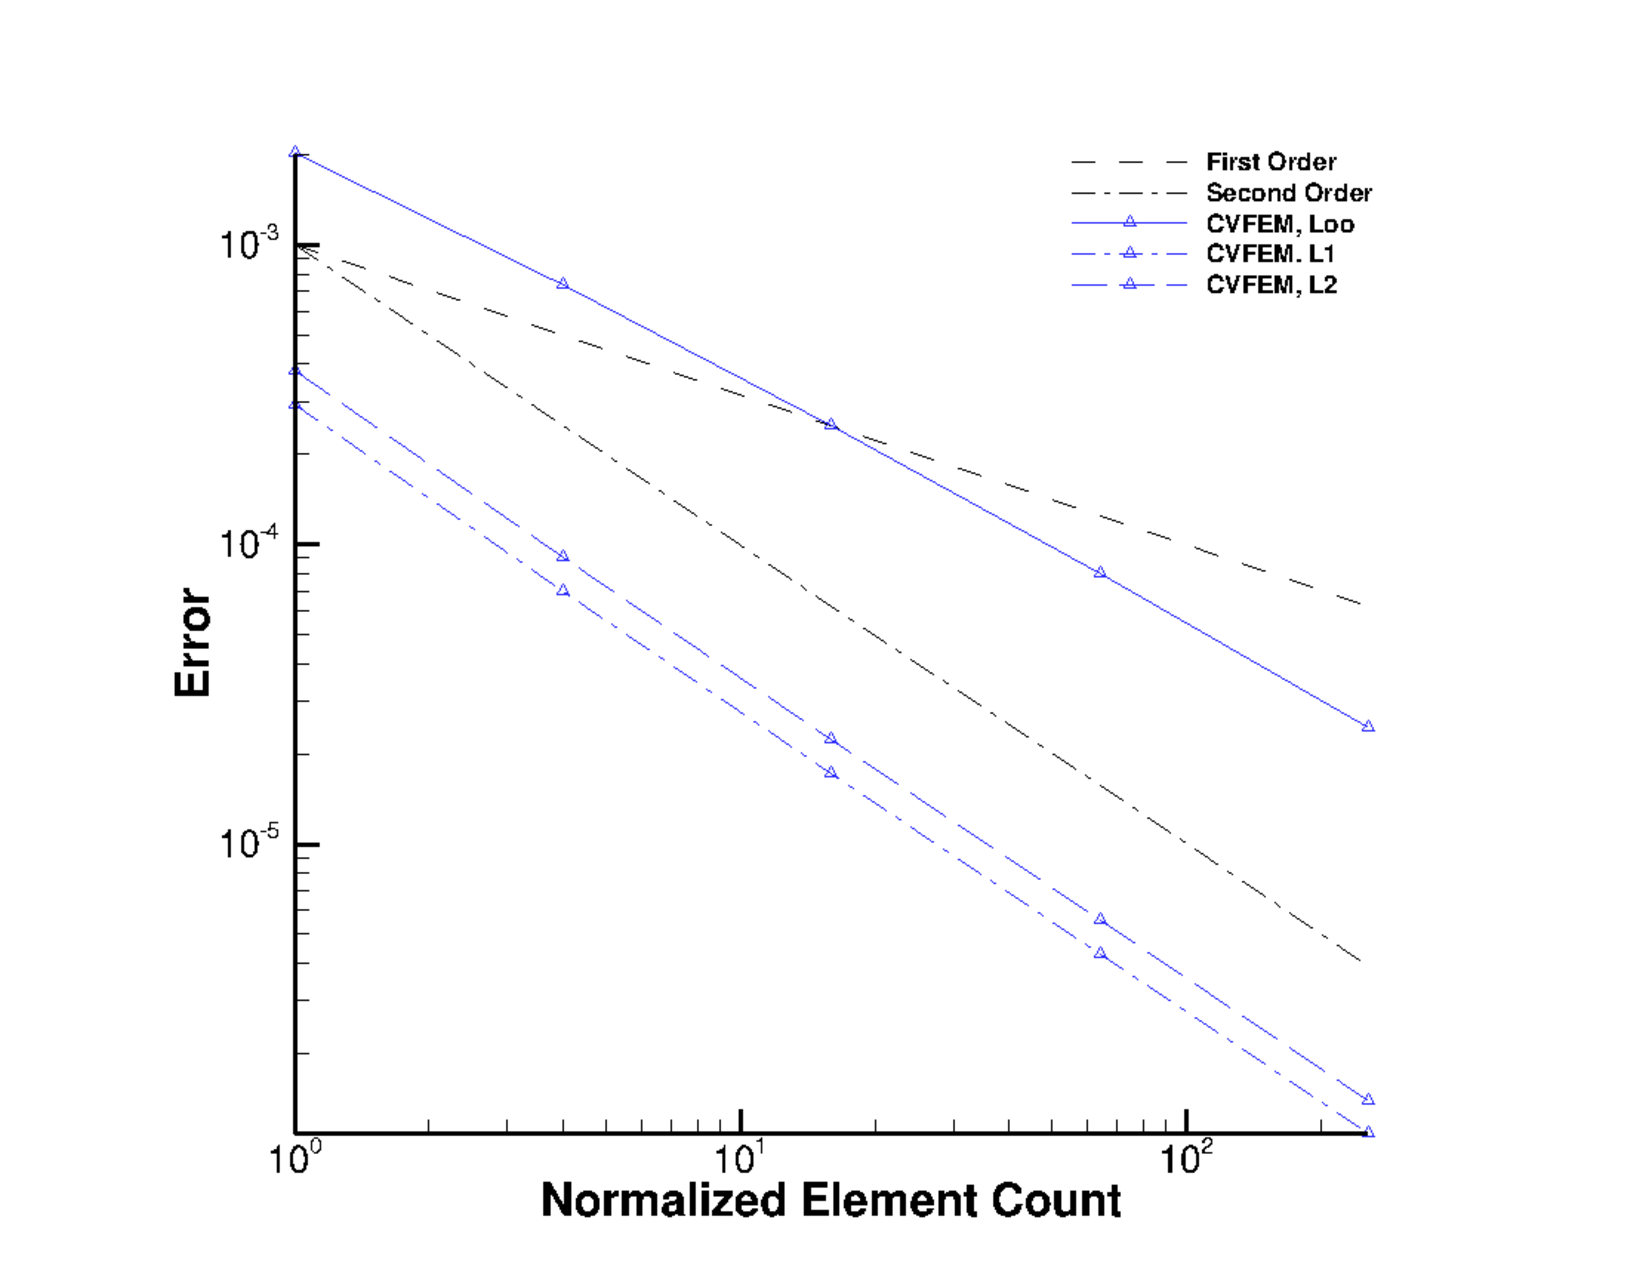
\includegraphics[width=0.8\textwidth]{figures/tquadLaplaceMMSCVFEM.pdf}}
  }
  \vspace{0.1in}
  \caption{Error norms for tquad4 refinement study.}
  \label{fig:laplaceTquad}
\end{figure}

An inspection of the magnitude of error between the exact and computed temperature for the R3 mesh is shown in Figure~\ref{fig:tquadTdiff}.
Results show that the CVFEM error is highest at the corner mesh nodes that form a reduced stencil. The edge-based scheme shows increased error
at the higher aspect ratio dual mesh. 

\begin{figure}
\centerline{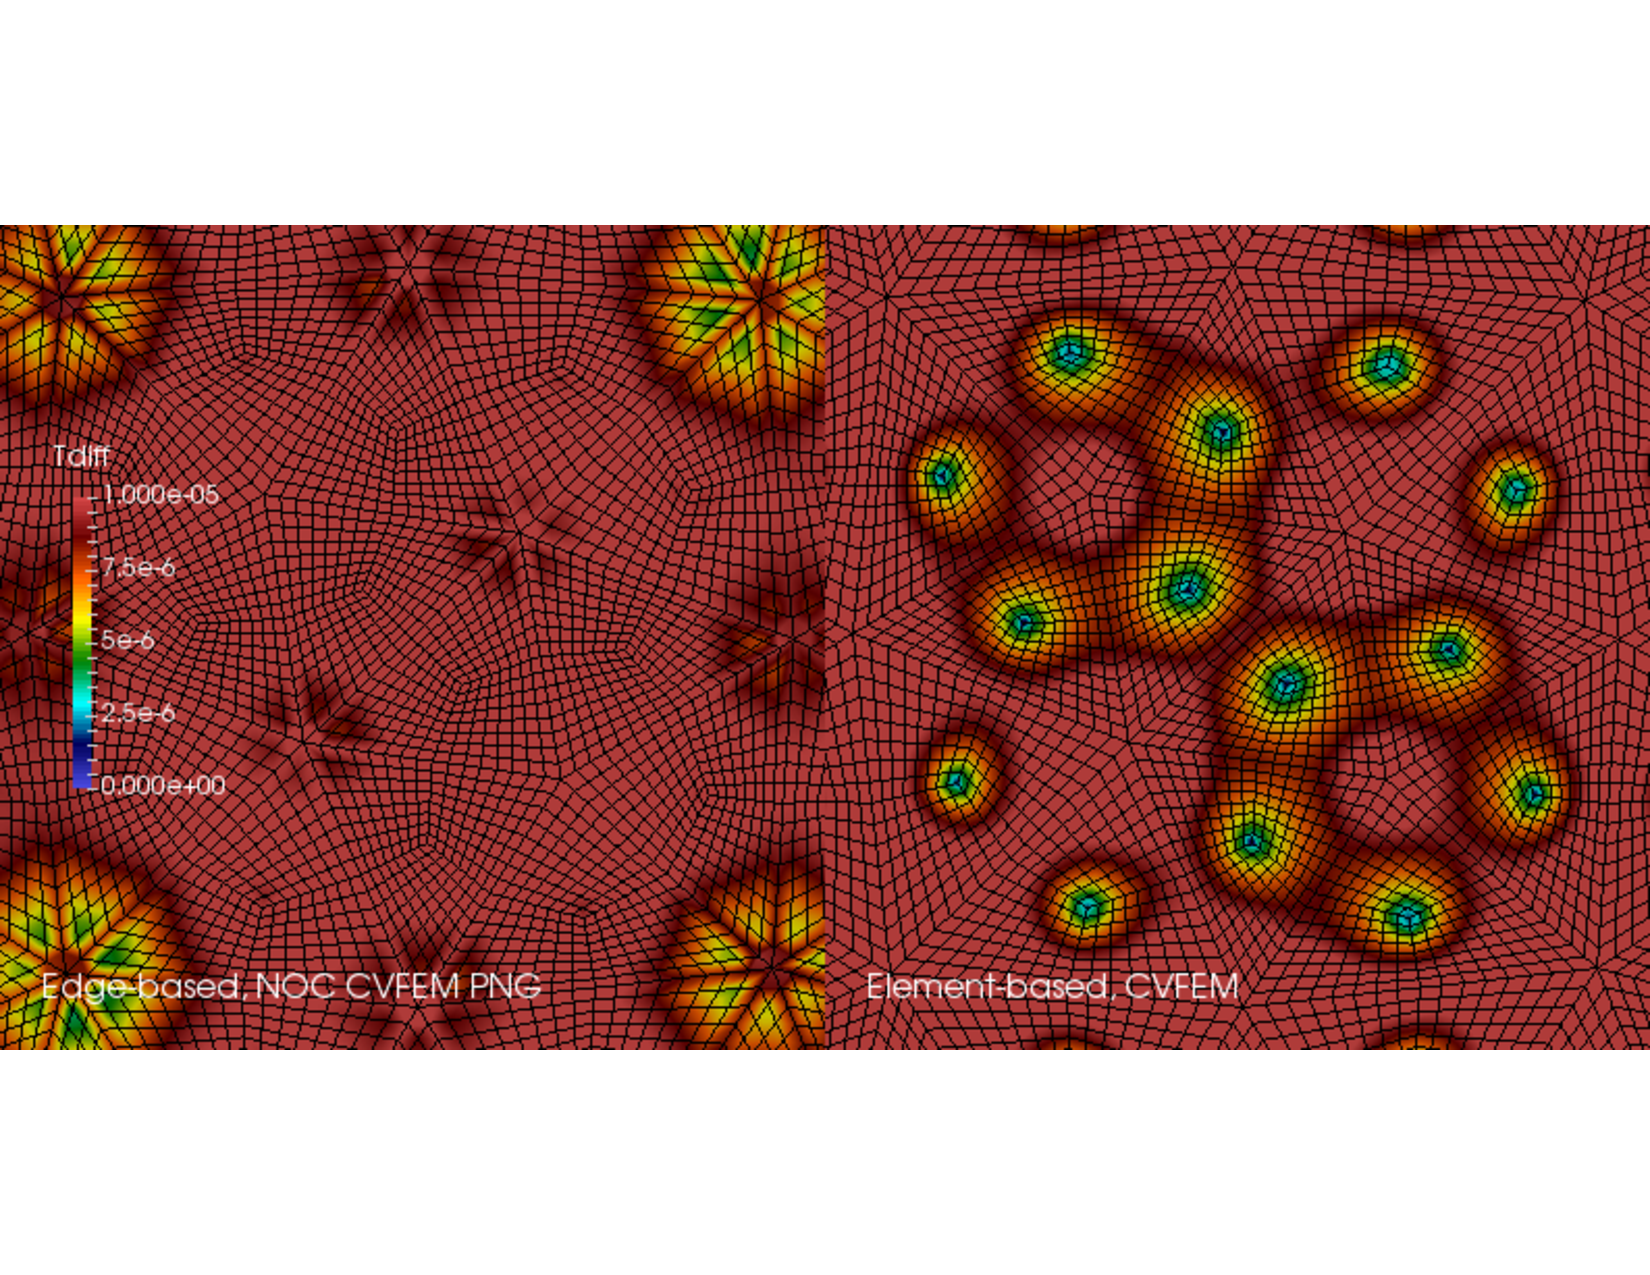
\includegraphics[width=0.8\textwidth]{figures/tquadEdgeCvfemTdiff.pdf}}
\caption{Magnitude of the $L_{oo}$ temperature norm comparing the edge-based CVFEM (NOC) and standard CVFEM operators on the R3 mesh.}
\label{fig:tquadTdiff}
\end{figure}

%%%%%%%%%%%%%%%%%%%%%%%%%%%%%%%%%%%%%%%%%%%%%%%%%%%%%%%%%
\section{3D Steady Laplace Operator with Nonconformal Interface}
%%%%%%%%%%%%%%%%%%%%%%%%%%%%%%%%%%%%%%%%%%%%%%%%%%%%%%%%%
A three dimensional element-based verification study is provided to evaluate the DG-based CVFEM approach.

\begin{equation}
  T = \frac{\lambda}{4} (cos(2 a \pi x) + cos(2 a \pi y) + cos(2 a \pi z)).
\label{3dT}
\end{equation}

Figure~\ref{fig:laplaceNC} represents the MMS field for temperature. The simulation study includes uniform 
refinement of a first- and second-order CVFEM basis. Both temperature field and projected nodal gradient
norms are of interest.

\begin{figure}
\centerline{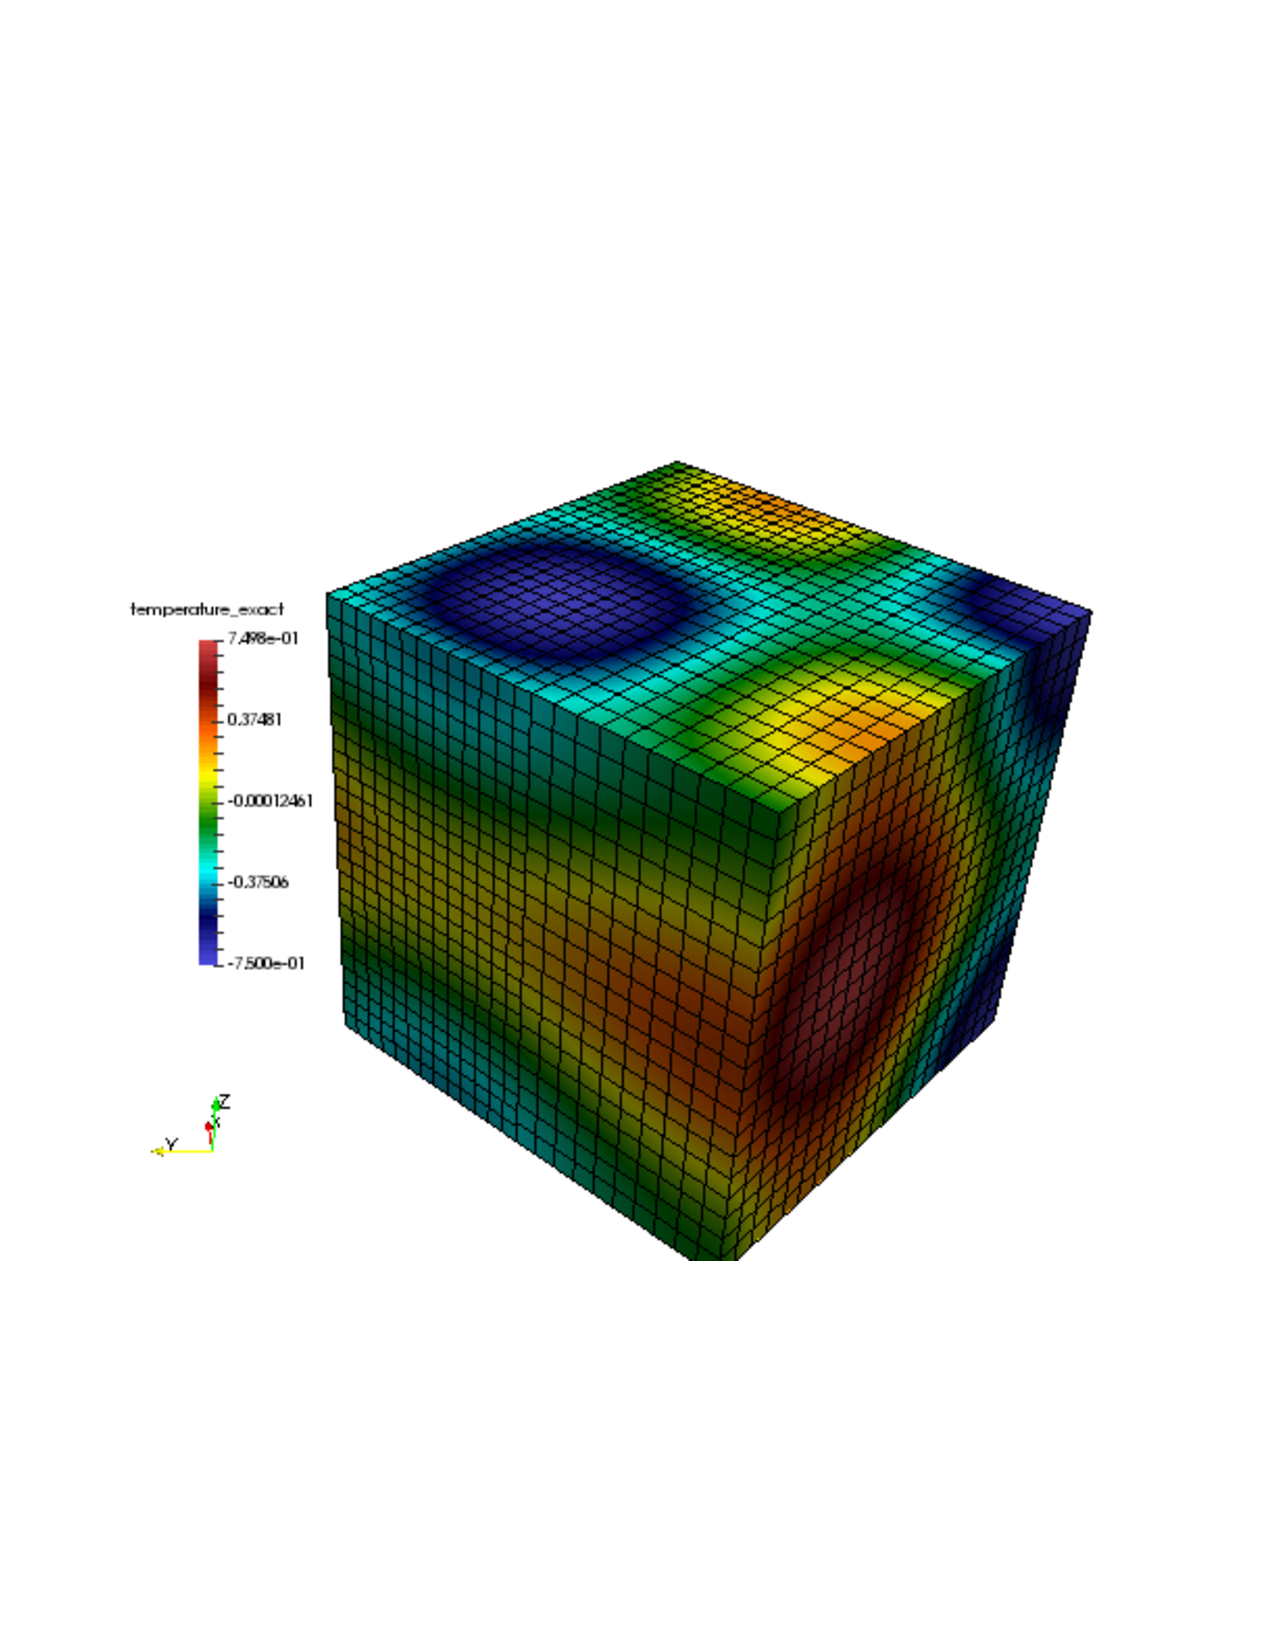
\includegraphics[width=0.8\textwidth]{figures/dgNonconformalCVFEM_3dTempMMS_tempField.pdf}}
\caption{MMS temperature field for nonconformal algorithm.}
\label{fig:laplaceNC}
\end{figure}

Figure~\ref{fig:laplaceNCOC} (a) outlines the linear and quadratic basis. For P1, the CVFEM temperature field predicts 
between second and first order while for P2, third order is recovered. When using a consistent mass matrix for 
the projected nodal gradient, second order is noted, see Figure~\ref{fig:laplaceNCOC}, (b).

\begin{figure}
  \centering
  \subfigure[Temperature norms for P1 and P2 elements.]
  {
    \centerline{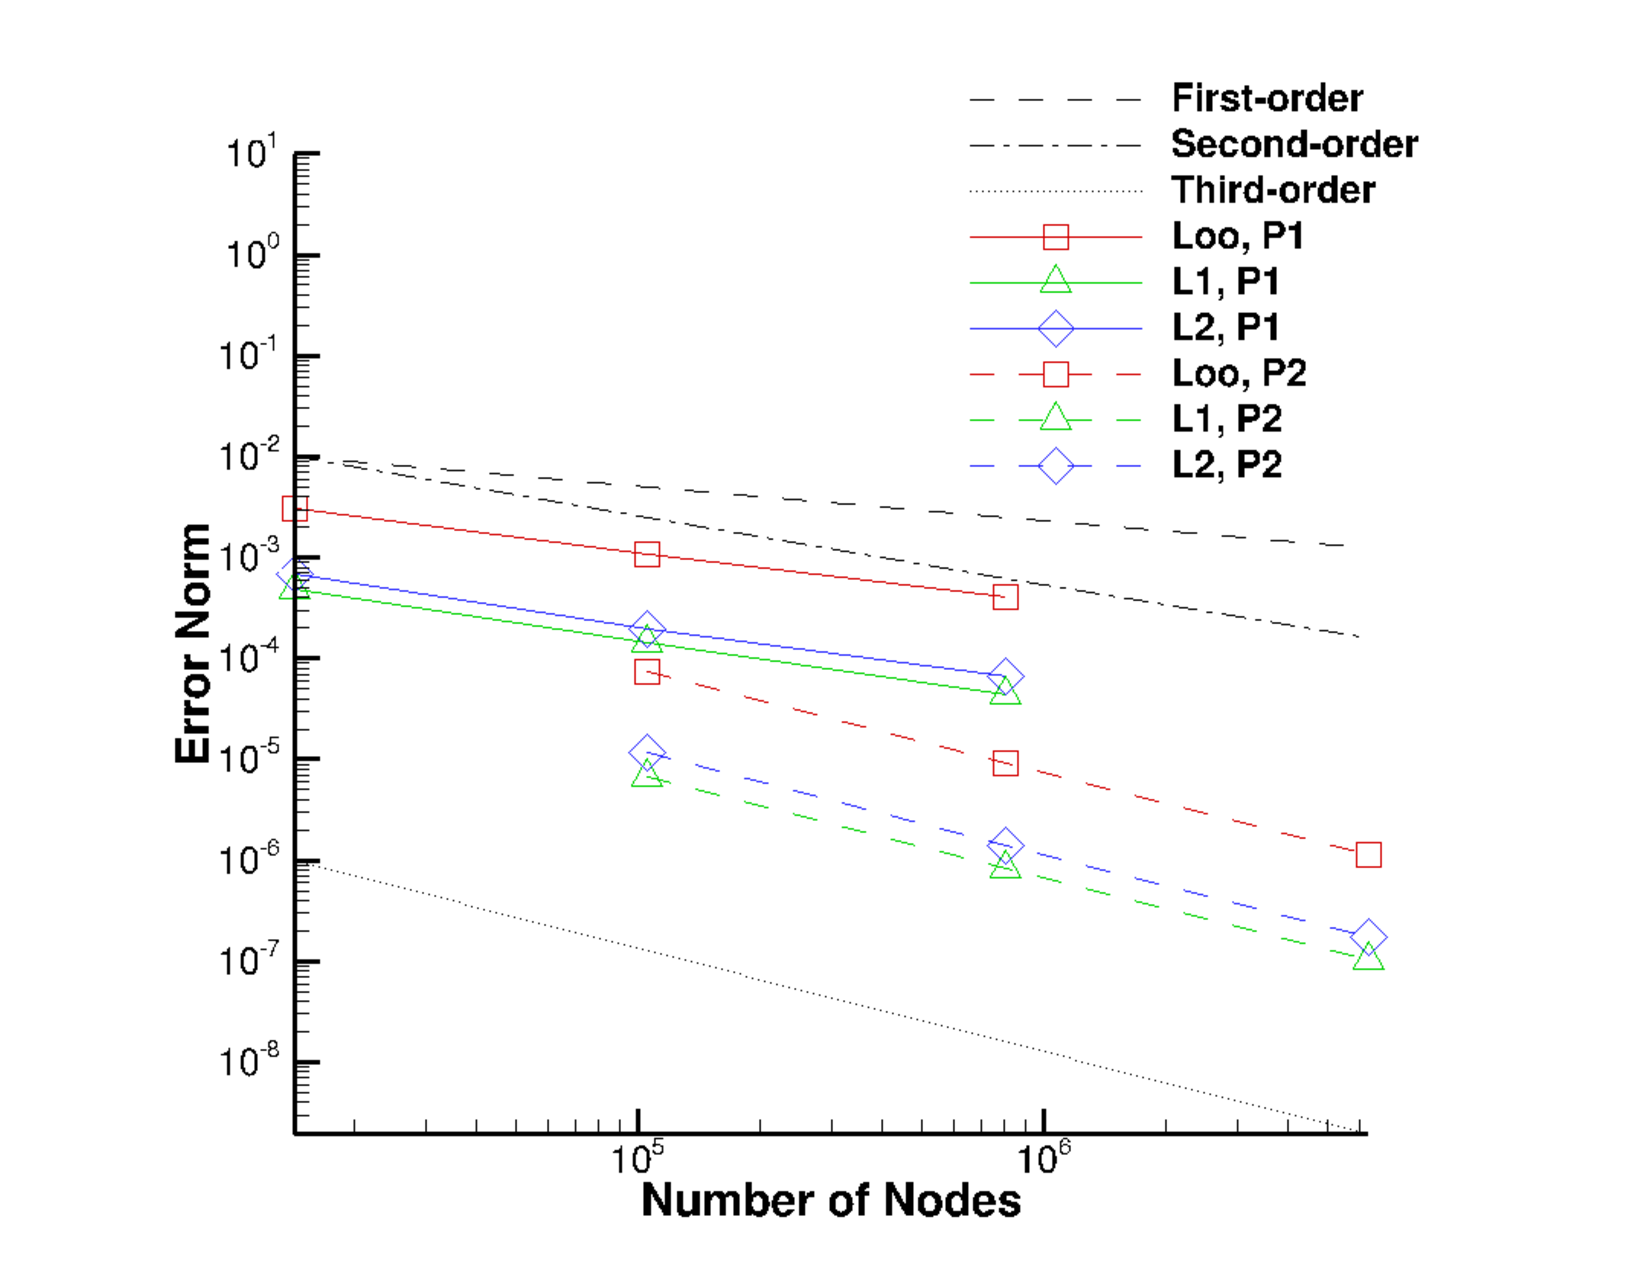
\includegraphics[width=0.8\textwidth]{figures/dgNonconformalCVFEM_3dTempMMS_OoC.pdf}}
  }
  \subfigure [Projected nodal gradient norms for P1 and P2 elements.]
  {
    \centerline{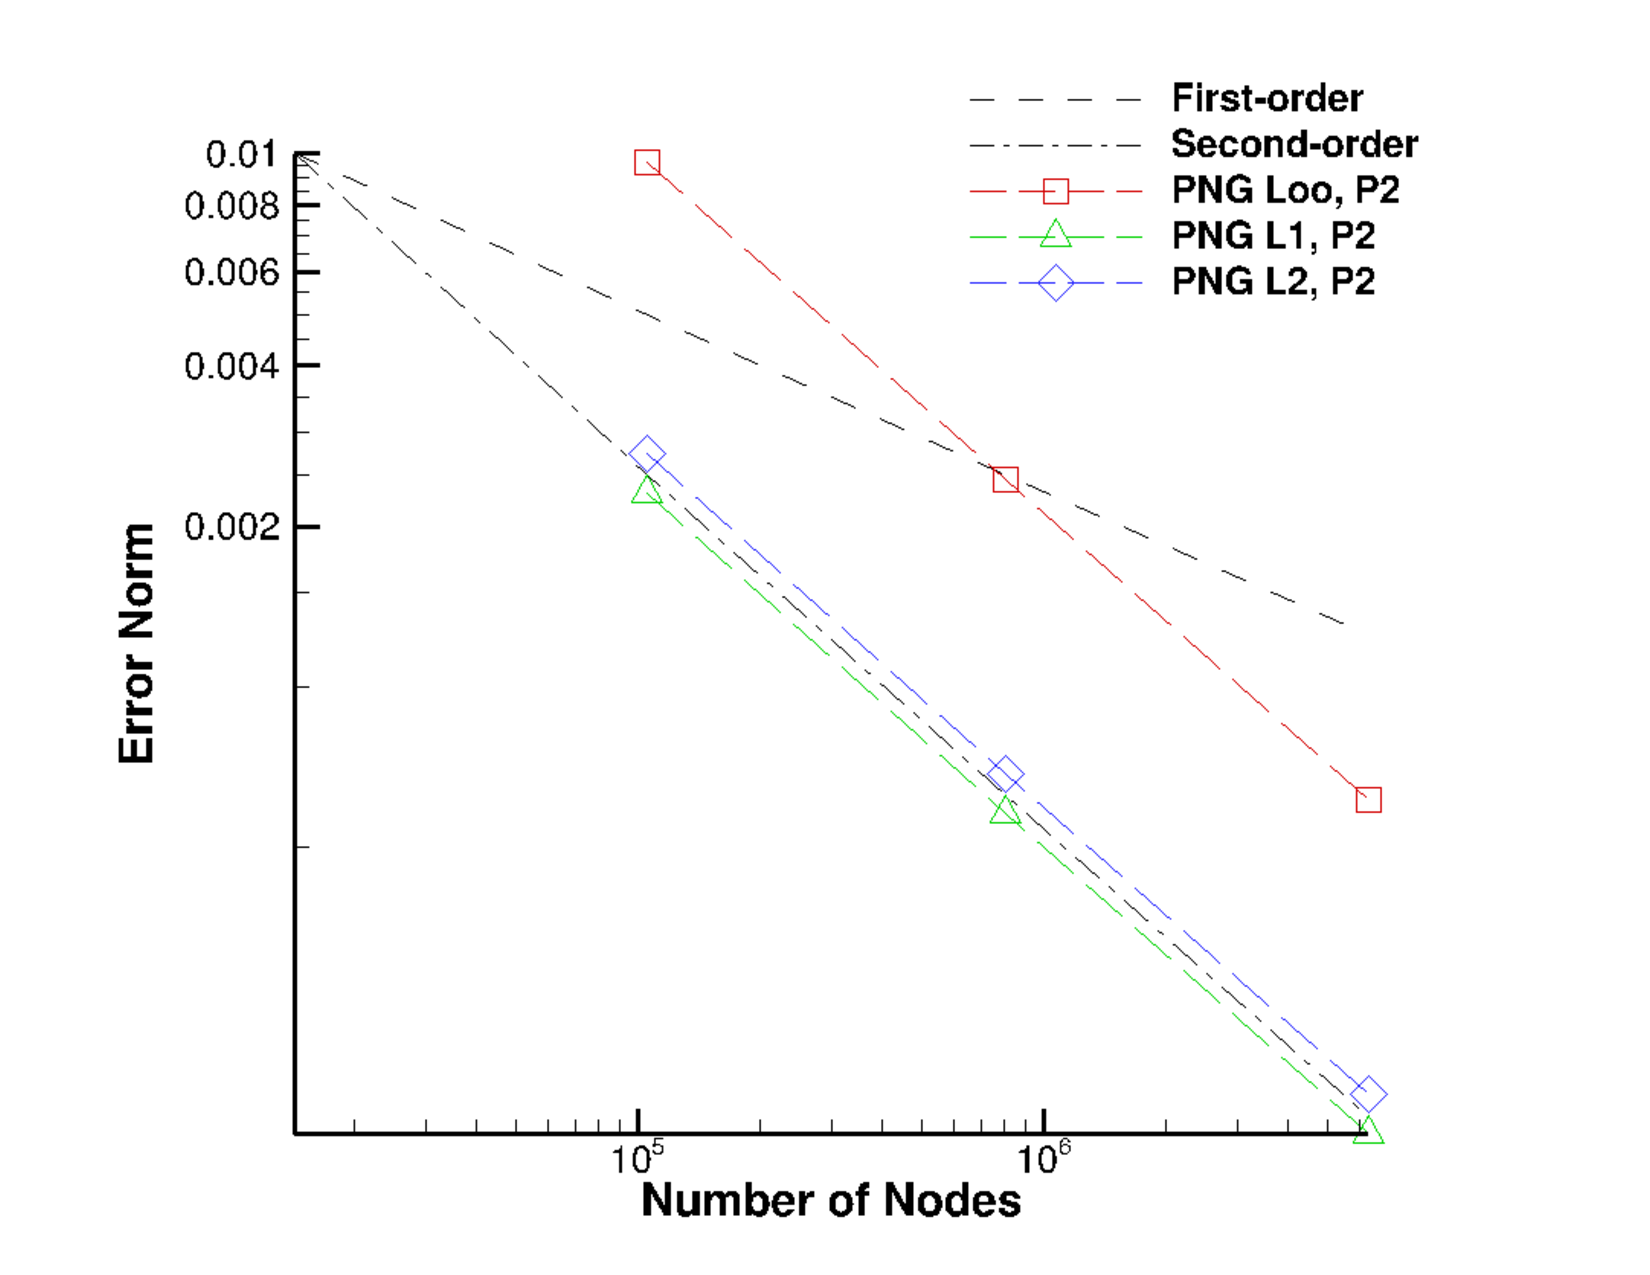
\includegraphics[width=0.8\textwidth]{figures/dgNonconformalCVFEM_3dTempMMS_OoCPNG.pdf}}
  }
  \vspace{0.1in}
  \caption{MMS order of accuracy for nonconformal algorithm.}
  \label{fig:laplaceNCOC}
\end{figure}

Given the order of accuracy results for the P1 implementation, a linear patch test was run. The temperature 
solution was simply, $T(x,y,z) = x + y + z$; all analytical temperature gradients are unity. Table~\ref{tab:linearPatch} 
demonstrates the successful patch test results for a P1 CVFEM implementation.

\begin{table}[h!]
  \centering
  \caption{Caption for the table.}
  \label{tab:linearPatch}
  \begin{tabular}{llll}
    dof & Loo & L1 & L2 \\
    \hline
    temperature & 3.33067e-16 & 2.30077e-17 & 4.68103e-17\\
     dTdx & 4.13225e-13 & 9.06848e-15 & 1.98249e-14\\
     dTdy & 4.15668e-13 & 1.11256e-14 & 2.15065e-14\\
     dTdz & 4.31211e-13 & 9.60785e-15 & 1.97517e-14
  \end{tabular}
\end{table}

 
